
\marginpar{Since these notes were designed to complement the lecture notes, I 
recommend you read those notes side by side with the lecture notes. The 
pagination of the slides corresponds to the lecture notes used in our year 
(2015-2016), the copy of those is hopefully still available at 
 \url{http://studentnet.cs.manchester.ac.uk/ugt/2015/COMP34411/COMP34411.pdf}}


\subsection{Converting source into meaning}
 The slides under the big Machine Translation title (p. 565-566) just 
 explain the logic of the English and Arabic sentences - ``The man wrote a 
 book'' and ``ktb Alrjl ktb'' which is the same thing in Arabic with some vowels
  omitted (this will be explained in the later sections of the handout).

Slide on p. 568 outlines the difficulty of mapping meaning to the target 
language, the language you are translating to.

The \texttt{[., (arg (claim)]} bits \marginpar{p. 571} are again the translation
 rules, corresponding to the two parse trees (drawn on the board during the 
 lecture):

\begin{center}
  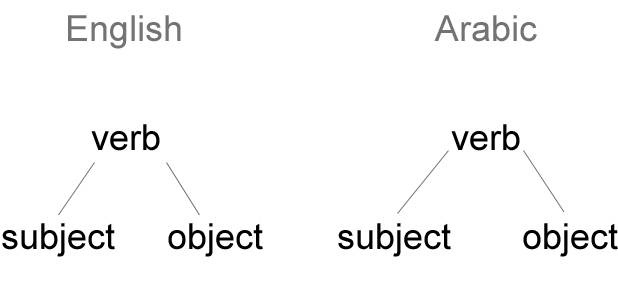
\includegraphics[width=0.4\textwidth]{images/mt-parse-trees.jpg}
\end{center}

So those rules just say to translate this sentence ``The man wrote a book'' into
Arabic.

OK, by inspecting the tree structure you probably would have guessed that if you
\textit{literally} translate from English into Arabic and the other way, speak 
like Yoda you will. \marginpar{my friend Google Translate thinks this is 
``The man writes  book''\ldots}  So the literal translation of, say, ``yktb 
Alrjl ktb'' would be ``Wrote the man book''. (literal translation + parse tree 
structure).

There are a few other catches to it. Arabic has the no indefinite article ``a''.
 Whoops. And also\ldots The definite article ``The'' is attached to the noun. 
 Instead of Al rajul (The man) they have ``Alrajul''. A bit like English has 
 sometimes ``doesn't'' or ``o'clock'' written instead of ``does not'', 
 ``on the clock''(is that even the correct version of o'clock?).

But that means the Arabic tree messes up, because it doesn't correspond
correspond to the English one (No ``a'', ``the man'' as one word\ldots). So, I 
think he discusses what to do to still make those trees align in the machine
translation. \marginpar{p. 573 onwards} We could treat ``Al'' as separate word 
for analysis, and then attach it on afterwards. But we will have to delete the 
indefinite article ``the'' to translate it into Arabic.

\subsection{Transfer rules} \marginpar{p. 575} 
This is where the actual transfer rule part starts (sort of). 
\texttt{[-def]} means the indefinite article. \texttt{[+def]} means the definite
 article. This, I am guessing is a representation of a sentence in a tree in a 
 flat form (``.'' is at the top, because he mentioned that the meaning of the 
 sentence changes with punctuation in some of the earlier lectures). Then we 
 have the verb and other things with articles attached (English: book has ``a'',
  man has ``the''. Arabic doesn't, but we sort of map them anyway - we know that
   ``book'' has ``a'' in English. In Arabic it doesn't, but that's where the 
   ``a'' would go if it was present in Arabic).

\marginpar{p. 576} Then we are shown the syntax, a nice and visual explanation 
below: 

\begin{center}
  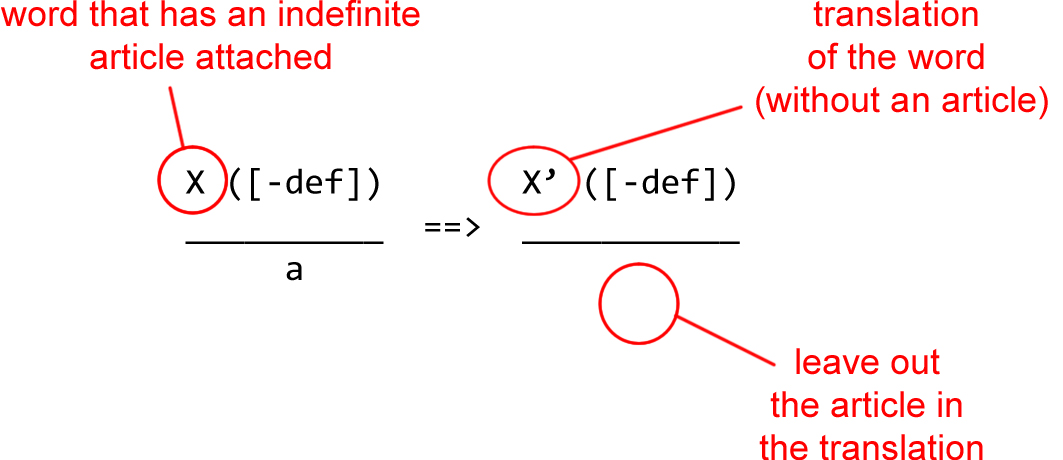
\includegraphics[width=0.6\textwidth]{images/mt-transfer.jpg}
\end{center}

 And apply this recursively to all of the English tree to get an Arabic one.

Start with applying all the little rules to all of the tree (word $\rightarrow$ 
word mappings, as far as I understood), then apply bigger rules (such as this 
one? I may be wrong in that specific part. He just said the bits not in 
brackets.)

\marginpar{p. 578 has the same thing with an auxiliary.} The thing is, English 
has more tenses than Arabic. So if you translate:

\begin{enumerate}
	\item English (source language): ``I am writing a book''
	\item Arabic (target language): ``I write a book''
	\item English (translated back from Arabic): ``I write a book''
\end{enumerate}

You see? The original meaning is lost! No problem when you translate \textbf{TO}
 Arabic. But when you translate \textbf{FROM} Arabic\ldots This is what he means
  in p. 580. The rules themselves though, allow you to convert sentence to tree 
  and backwards - tree to sentence.

\marginpar{p. 581} He carries on with the point he made earlier - what if one language has
distinctions the other one doesn't. He gives you the example of ``they''.
Russian also has a single, gender-neutral form ``oni'', so I was puzzled to find
about those distinctions. French has ``ils'' and ``elles'' for plural masculine 
and plural feminine forms, Arabic, as well as having those two gender 
distinctions also distinguishes whether there are two of them (the people you 
are referring to) or more than two.

So again, when you have to translate - part of the meaning can get lost:

\begin{itemize}
	\item \textbf{John and Mary went to the cinema. They enjoyed the picture.}\\
	Here we know from the surrounding context that we have a male and a female. 
	So to translate that we use plural masculine of ``they'' (because if at 
	least one person is a male - masculine form is used. This is true in all the
	 languages I studied that make that distinction), representing 2 people for 
	 Arabic.
	\item \textbf{Sam and Alex went outside. They enjoyed the sun.} \\Here two 
	gender-neutral names are used. How the heck are you supposed to know what 
	form of ``they'' to use now? Only if you have more surrounding context, if 
	you don't - Houston, we have a problem!
\end{itemize} 

Also, earlier tense distinctions still apply here.
(He is so correct about the bare plural!!!)

\marginpar{p. 584} Here he explains how some things don't map to other languages as a single
word. ``I am looking for a unicorn'' translates to French as ``I am in search of
a unicorn''

``looking for'' (2 words) $\rightarrow$ ``in search of'' (3 words)

The opposite is true for English. You can say ``We dined'' but you don't say
``We breakfasted'', ``We tead'' (as opposed to ``we had breakfast'', ``we had
tea'') and you don't really say ``We lunched''. Some languages have (Russian
definitely has) them all as verbs.

For idioms, even if an idiom with an equivalent meaning exists you still
translate it as a bare meaning (at least according to Allan, I clarified).

So if you have ``kick the bucket'' in English and say you want to translate it
to Russian, instead of using the equivalent phrase (``kon'ki otbrosit'',
literally translates as ``throw away the ice skates'') you translate it as
``become dead''.

\subsection{The MT pyramid} 
\marginpar{p. 586}

The gist here is the fact that no matter what language you use (out of the ones
we studied) you have the same parts of speech. You say ``I'', ``je'', ``ich'',
``ya'', ``watashi'' or ``he'', ``il'', ``er'', ``on'', ``kare''\ldots you know 
they are pronouns. Doesn't matter what language, it's a pronoun! That's an
interlingua.

Another example of interlingua: transitive verb with subject and object becomes
a transitive verb with subject and object.

Interlingua is very general.

\marginpar{p. 591} (as far as I understood from there)  
\textbf{Textual entailment vs machine translation:}\\ 
in textual entailment you use logic to figure out the links:

John and Mary got divorced $\rightarrow$ John and Mary were once married.

Machine translation - you map from one language to another, preserving the gist.
Text simplification can also be interpreted as translation \marginpar{Wikipedia:
English $\rightarrow$ Simple English!}

\subsection{Ambiguity in MT} 
\marginpar{p. 592}
There are 3 kinds of ambiguities mentioned. 
\subsubsection{Structural ambiguity}

\begin{itemize}
	\item \textbf{strawberry jam jar}\\ 
	Ok, that's pretty obvious. It's a jar of strawberry jam! Think again. They 
	are 3 nouns. Machine can't just say what you just said. Machine needs to 
	know whether it is \textbf{(strawberry jam) jar} or \textbf{strawberry (jam 
	jar)}

	Basically which two nouns to group to get the right meaning. For humans it 
	is not such a big deal. Other languages (Dutch):

	\textbf{aardbeienjam jar}

	The words that need to be ``bracketed'' are just mashed together!

	\item \textbf{I saw a man with a telescope.} Did you use a telescope to see 
	the man? Did the man you saw have a telescope with him?
	\item \textbf{Purple cake-eating monster.} Is the monster purple? Or does it
	 eat exclusively purple cakes?
\end{itemize}


\subsubsection{Scope ambiguity}

\marginpar{This one was trickier (at least for me). So I suggest you watch this 
video: \url{https://www.youtube.com/watch?v=XC-MGuj75zQ} This guy will probably 
explain better than me. The next few lines are essentially a TL;DR of the 
video.}

Basically we use quantifiers in our speech. They are not obvious, because our
mind works differently from a machine.

Any, every, a\ldots

These guys map to ``there exists'' and ``for all''. UBIQUITOUS LOGIC!

All John's friends went to a fantasy land.

There are two meanings:

\begin{enumerate}
	\item ``All John's friends went to the same fantasy land.''
	\item ``All John's friends went to different fantasy lands, it's just for 
	every friend there exists a fantasy land they went to - Sarah went to Oz, 
	Stephen went to Narnia''
\end{enumerate}

The first meaning comes from ``all'' friends (``all'' winning over ``a''), that
is for each friend there exists a single one fantasy land that is the same for
everyone.

The second meaning comes from ``a'' (``a'' winning over ``all'') - for each
friend there exists a fantasy land, which does not have to be the same fantasy
land.

Then he goes on to explain how does our brain pick the first interpretation,
even though the second one is more logical.

\marginpar{TL;DR ends}

The 2 examples Allan gives in the lectures - one about John drinking, another 
one about searching the unicorn.

\subsubsection{John will drink everything}
The distinction between any and every is subtle. Sure, they are both universal
quantifiers, but what exactly is their difference in scope? Consider:

\begin{itemize}
	\item You can't invite John. He will drink EVERYTHING.
	\item You can't invite John. He will drink ANYTHING.
\end{itemize}

That is (WARNING: over-complication coming through):

\begin{enumerate}
	\item John will drink \textbf{EVERYTHING.}\\ There exists \textbf{ONE} 
	situation where he will drink ALL the drinks.
	\item John will drink \textbf{ANYTHING.}\\ Whatever you offer John, there 
	exists at least one situation where he will drink it. Total: \textbf{MANY} 
	situations, many possibilities. 
\end{enumerate}

\subsubsection{The unicorn example}
This one was not obvious to me.

The ambiguity comes from whether there actually exists a unicorn John is looking
for or does it not exist? This can be interpreted in two ways:

\begin{enumerate}
	\item John is looking for a unicorn. Don't tell him they don't exist.\\
There \textbf{ISN'T} a unicorn John is looking for.
	\item John is looking for a unicorn. It ran off the castle this morning. \\
There \textbf{IS} a unicorn John is looking for.
\end{enumerate} 

\marginpar{A nice procrastination 
source: 
\url{https://en.wikipedia.org/wiki/List_of_linguistic_example_sentences}}
\subsubsection{Lexical ambiguity}
When you have a word with several meanings and you don't know
which one is intended. The word ``bank'' is one such example.


\subsubsection{Which one has the biggest impact?}
\marginpar{The sign above the fire extinguisher has two inscriptions above it, 
written in 2 languages. The top one is in Chinese and below is an English 
translation. The English translation proudly read: ``Hand grenade''}
So, from language to language structural ambiguity (not always, but sometimes)
and scope ambiguities transfer. Lexical ambiguity doesn't.

But it is the lexical ambiguity that causes the most pain, since if in the 
source language has the word with several meanings, and it is not obvious from 
the surrounding context what meaning to use\ldots 


\subsection{Bilingual corpora, parallel corpora} 
\marginpar{p. 597}

Here he just talks about how can he literally compare words side by side with
some adjustments. He will match two words if they are in the same
position/roughly the same number of consonants/all this bunch of rules
together/etc.


\subsection{Alignment} 
\marginpar{p. 604 onwards}

Because of the word order he will have to use a thing similar to string-edit
distance to be able to do that - insert a word on one language, delete on
another one.

professor of formal linguistics $\rightarrow$ professeur de linguistique 
formelle.

Insert ``formal'', delete ``formelle''.

He then proceeds to talk about the dynamic time warping algorithm, mentioning 
what happens if he deletes all the words that match with their positions. He 
will get some unmatched ones and he can reasonably match the unmatched ones by, 
for example, looking at their lengths.

There are still problems: \marginpar{p. 611}
\begin{itemize}
	\item If one language distinguishes things the other one does not, such as 
	the definite article ``the'' translates to ``le'' for masculine, and ``la''
	for feminine.
	\item English has bare plural Noun Phrases, so ``precise formal 
	descriptions'' does not have an article in front of it, like French does:
	``\textbf{des} descriptions formelles precises''.
	\item Lexical ambiguity - French has two words to represent ``language'':
	``langue'' and ``langage''. 
	\marginpar{This explains the differentiation really well: 
	\url{http://awesomefrench.tumblr.com/post/55078404181/difference-between-langue-langage}}
	Basically ``langage'' can mean slang or jargon, etc.\, it's the general way 
	we speak. ``Langue'', on the other hand means the group of languages with 
	the same grammar rules. English is a ``langue''. Indo-european languages are
	``langues''. This really messes the alignment up. Say 30\% it would map to 
	``langue'' and 70\% to ``langage''!
	\item Different languages have different sentence structures. So ``natural 
	language'' translates as ``langage naturel''. See how words changed round?
\end{itemize}

\marginpar{p. 612 onwards}
Then he gives an example of Qur'an and how can it be used to align words. The 
difficulty comes with words like ``book'', because by adding affixes onto the
word you can get it to mean ``of his book'', ``and the book'', etc.

\marginpar{See the rest of the notes for some unusual matches.}
One strategy to translate the passages would be to make the following 
assumption: a translation ought to occur the same number of times as the word it
 is translating. So multiply the word count by ratio of word in source language 
 and word in target language ($W^S$ and $W^T$). 

 The following improvements can be made: \marginpar{p. 623}
 \begin{itemize}
 	\item Block the target translation ($W^T$) as the translation of the source 
 	word ($W^S$) if you have already used it as the translation of a different 
 	source word ($W^{S'}$)
 	\item Use part of speech tags - match words with the same POS tags. But 
 	there is also ambiguity: ``I ran to the station'' in Spanish. \marginpar{If 
 	someone knows where the ambiguity comes from, I would be grateful if you 
 	tell me!}
 \end{itemize}


